%!TEX root = series of tubes.tex
\begin{figure*}
\centering
    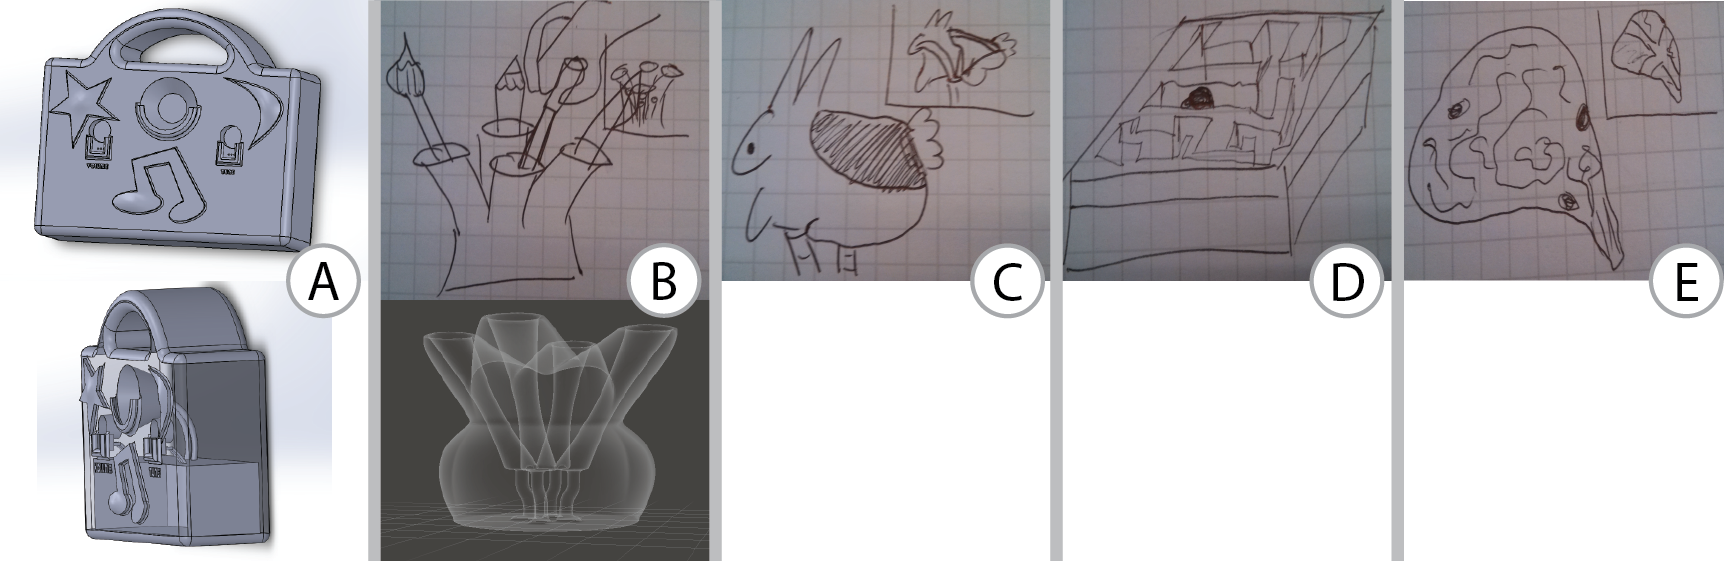
\includegraphics[width=7in]{figures/examples.png}
\caption{A series of example objects created using our system.  (a) is a touch-sensitive brain toy.  (b) is a rabbit which ``breathes'' using wind pipes we built.  (c) shows a portable radio.  (d) shows a presence-aware pen holder.  (e) is a maze game.}
\label{fig:examples}
\end{figure*}

\section{Example Objects}
\bjoern{subsection headings need to be updated in light of the simplification and label changes in the design space.}
To evaluate and highlight our tool's capabilities, we fabricated a set of five prototype objects designed using \systemnamenospace.  All prototypes were fabricated in a single piece, unless described otherwise. \bjoern{2 of 5 will have been fabricated otherwise -  Radio, Neon sign - both in pieces.}

\subsection{Touch-sensitive Toys (open, liquid, star, terminals)}

To show how conductive fluids can be used for touch sensing, we created a set of touch-sensitive toys and a companion app that identifies the objects as well as touched parts of the objects (inspired by \cite{Harrison-acoustic}). The objects --- a brain and boat, in our example --- can be set on a base, upon which a speaker announces ``brain'' or ``boat''. Touching the brain model's front protrusion yields the announcement ``olfactory bulb''. The distinct touch points on each object are connected by an interior star topology, and touch sensing is performed via a single conductive connection to the base, using swept-frequency capacitive sensing~\cite{Sato-touche} (see Figure \ref{fig:toys}). %We built a smart base which can distinguish between the toys and also determine which toy is mounted:
Since each toy and each gesture has a distinct capacitive signature, we use a simple classifier trained to detect both toy and gesture based on profile.

The models we used for the toys' exteriors were all downloaded from the free website Thingiverse.  All components were fabricated on a Makerbot, support-free.  After printing, we injected copper paint (CuPro-Cote) into the interior pipes using a craft syringe.  This paint requires approximately 2 days to fully dry in this configuration (3mm diameter tubes, maximum tube length 10cm).  Our smart base is powered by an Arduino Uno running open-source SFCS code\footnote{http://www.instructables.com/id/Touche-for-Arduino-Advanced-touch-sensing}.

\subsection{Breathing Bunny (semi-closed, gas, terminals)}

To demonstrate how gases can be used to both provide sensation to the user through openings and to deform a model internally, we created a rabbit with a pair of tubes that can simulate breathing (see Figure \ref{fig:breathe}).  When the rabbit inhales through its nose, its abdomen rises, and as it exhales its abdomen falls.  For this, we used a combination air/vacuum pump: one terminal creates a vacuum while the other creates positive pressure.  Our rabbit has two pipes, one open tube exiting at its mouth and one semi-enclosed, capped pipe capped in its abdomen.  We connected one pipe to each of our pump's terminals, and using a programmable power supply we mimic a rabbit's breathing pattern.  This example was printed on our Objet in rubberlike material, with support flushed post-print.

\subsection{Custom Radio (open, threadable, terminals)}

A custom radio shows how pipes can be used to integrate electronic components into the user-facing surface of an object. This device uses a network of disconnected open pipes threaded with wires to connect our components (two potentiometers, an LED, and a speaker) to a microcontroller (Arduino Pro Micro). We placed the microcontroller, an Si4703 radio tuner breakout board and a battery-driven power supply in the base of the radio. 

This design with 8 pipes (3 per potentiometer, 1 for the LED, 1 for the speaker) showed the limitations of our incremental routing strategy: since we voxelize and remesh for each pipe, surface detail is incrementally lost. The problem can be addressed by increasing the voxel resolution. At 512x512x512 voxels, surface geometry is not notably degraded. However, a single cut operation takes around 3 minutes \bjoern{on what hardware? mention earlier}, compared to near-instant performance on a $128^3$ voxel grid.  We fabricated the radio itself on our Makerbot, support-free but cut in two pieces to allow the Arduino and battery pack to be inserted.

\bjoern{I ran out of steam somewhere here...}
\subsection{Presence-aware Pen Holder (open, solid, ternimals)}
\bjoern{isn't this a threadable instead of a solid?} \bjoern{the model looks like the acutal pipes are really short and basically straight at the bottom of the model. This may raise the question if one couldn't just use the line sensors without any fiber optic cable in the middle.}
Our presence-aware pen holder can distinguish which tool or tools a user has picked up (see Figure \ref{fig:pens}).  Our pen holder uses a modification of the FlyEye technique described by Wimmer in \cite{Wimmer-flyeye} in which \bjoern{describe...}. Four internal pipes are threaded with fiber optic cables, one per pen chamber.  We use a single cable per chamber; our 6mm diameter fiber optic cables, in comparison to the fine tubes used in the original work , can send and receive through the same cable. \bjoern{is this because it has many strands?}  At the base of each tube is a QRE1113 line sensor digital breakout board, which has an integrated IR emitter and receiver.   When a pen is in its appointed place, the emitted infrared light is reflected off its bottom and travels back to the receiver, where it registers as bright.  This prototype was built by our Objet and support was flushed post-print.\bjoern{Incorrect. Looks like a Makerbot print.} \valkyrie{this whole paragraph is unclear}

\subsection{Animated Neon Sign (return, threadable, path)}

\begin{figure}[h!]
\centering
    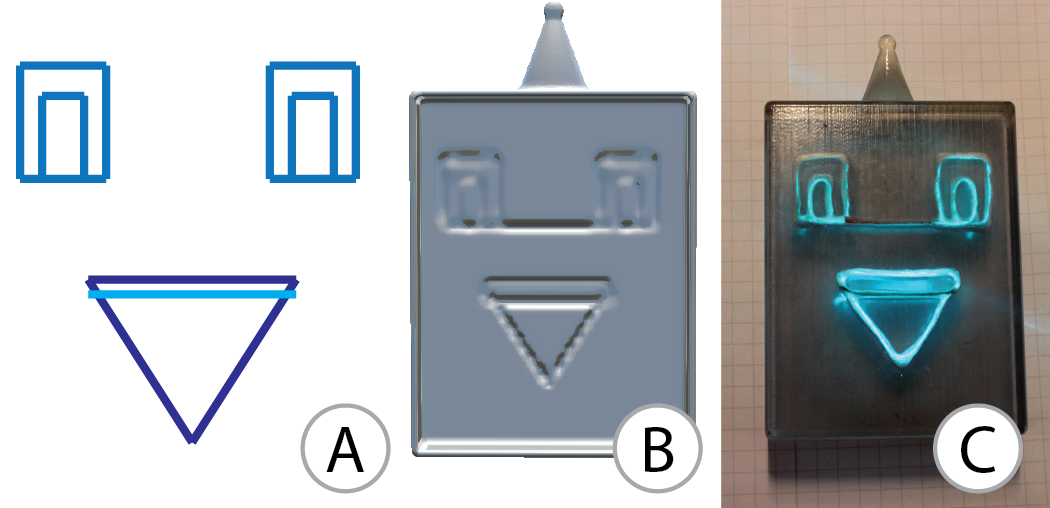
\includegraphics[width=3.4in]{figures/sign.png}
\caption{A two-state animated neon sign designed using our tool.  (a) shows the input SVG files, with the two states of the mouth drawn in different colors. \bjoern{it's hard to tell these colors apart!}  (b) shows the resultant mesh when we subtracted the generated tubes. \bjoern{hard to see what's going on here, too.} In (c), we show the fabricated sign.}
\label{fig:neon}
\end{figure}

Neon art, perhaps best known for its association with Las Vegas, is traditionally made from hand-formed glass tubes containing neon gas.  The tubes light up when a current is passed through them.  For this type of art, the path of the tubes is of crucial importance, as it determines how the sign will look.  We designed a custom neon robot head which can be animated to ``talk''.  The pipes have been threaded with electroluminescent wire which is lit in sequence to create an animation.  Our sign was fabricated on the Objet in two halves, cutting through the plane of pipe path to facilitate assemblhy. Pipes enter and exit through the rear to hide the EL wire controls.  The EL wire was threaded post-print, and is controlled by an EL wire sequencer.

\subsection{Maze (fully enclosed, particulate, tree, terminals + path)}

Using a modification of our graph-based algorithm which only cuts the literal drawing (and does not perform Eulerization, etc.), we created a maze game with a single particle trapped in a fully enclosed tube.  This maze is based on an SVG we created by hand and processed with our internal path tube tool.  To fabricate the tube, we created it in two halves that were fastened together via glue, due to limitations in our ability to remove support material otherwise (we only have access to a high-pressure water tool, not a lye bath).  We created this prototype on our Objet in two halves, inserting a marble before closing. \bjoern{check - i think the latest maze is in fact done with our tool? Will need rewriting.}